\documentclass[12pt]{article}
\usepackage[backend=bibtex, sorting=none, giveninits=true, doi=true, url=true, maxbibnames=3]{biblatex}
\usepackage{times} 
\usepackage{titling}
\usepackage[paperheight=11in, paperwidth=8.5in, left=0.75in, right=0.75in, top=1.00in, bottom=1.00in]{geometry}
\usepackage{authblk}
\usepackage{graphicx}
\usepackage[labelfont=bf, labelsep=period]{caption}
\graphicspath{ {./images/} }

\setlength{\droptitle}{-8ex}
\pretitle{\begin{flushleft}\large\bfseries}
	\posttitle{\par\end{flushleft}}
\preauthor{\begin{flushleft}}
	\postauthor{\end{flushleft}}

\pagenumbering{gobble}
\setlength{\parindent}{0pt}
\setlength{\parskip}{1em}

\addbibresource{mmMeetingBibliography} 

\renewcommand\Authfont{\fontsize{12}{12}\selectfont}
\renewcommand\Affilfont{\fontsize{12}{12}\selectfont}

\author[1]{First Author}
\author[2,*]{Second Author}
\author[1,3]{Third Author}
\affil[1]{Affiliation of the first author, Department/Institution, City, State/Province, Country.}
\affil[2]{Affiliation of the second author, Department/Institution, City, State/Province, Country.}
\affil[3]{Department of History, University of Illinois – Urbana-Champaign, Urbana, IL, United States.}
\affil[*]{Corresponding author: SAuthor@prydonian.edu }
\date{\vspace{-5em}}                     

\title{\vspace{-1.5em}The Title Should Be in Title Case (See Below), Single Spaced, Times New Roman, Bold 14-point, Left-justified, with a Maximum of 300 Characters or 75 Words{\vspace{-0.7em}}}

\begin{document}
	
\maketitle

The paper should be a condensed version of your presentation and include all significant findings. Write the text so that readers who are not specialists can appreciate the purpose of the study and understand the procedures and conclusions. The text, entirely written in English, should include a brief introduction and motivation of the study, including experimental procedures, main results, and conclusions. It is not necessary to divide the text into sub-sections, except for the References section.

Capitalize all major words in your title as shown in the example above (nouns, pronouns, verbs, adjectives, adverbs, and some conjunctions). Use lowercase for articles: the, a, and an; for the following conjunctions: and, but, for, or, and nor; for the part of a proper name that would be lowercased in the text, such as de or von; and for the second part of a species name, such as fulvescens in Acipenser fulvescens, even if it is the last word in a title or subtitle.

Your paper must be submitted as an editable word processing file (preferably Microsoft Word) in .doc or .docx formats. Use a 12-point Times New Roman typeface and single spacing between lines. Use italics for taxonomic terms. Avoid individualized formatting and special typefaces. Document size should be 8.5 x 11 inches (21.59 x 27.94 cm), with margins of 1.0 inch (25.4 mm) top and bottom and 0.75 inch (19.1 mm) left and right. The body of the text (i.e., excluding title, authors, affiliations, references, and figure caption) should be full-justified and between 400-6000 characters. Papers with character counts outside of this range will be rejected. Skip a line before each new paragraph, but do not indent paragraphs. 

Figures are NOT required for regular submissions, but submissions applying for a Meeting Award are required to have two figures. Include figure labels and scale markers on all figures. Captions should be placed below all figures and tables. Artwork and tables must be electronically inserted into the document. Color figures may be used and will be reproduced in any electronic proceedings distributed. If printed, paper copies will be in grayscale, so ensure that color coding used for legends is distinguishable in grayscale. Line art must be created either in drawing software or scanned into a suitable format for importing into the document. Check that the line widths and font sizes allow the figure to be clear at its final size.

References should be included at the end of the text, with the appropriate reference styles for journal articles\cite{article1, article2}, books\cite{book}, conference proceedings\cite{proc1}, and websites\cite{webpage}. Indicate references within the text with Arabic numbers in square brackets, preferably at the end of the sentence, before the period. For references with four or more authors, use the first-named author followed by “et al.”. Acknowledgements, statements regarding of the division of work, or disclaimers should be included in the last reference, which is cited at the end of the last sentence of the text.
All submissions are reviewed by the Program Committee according to the following criteria: (a) relevance to a specific symposium, (b) scientific content, quality and innovative proposals, (c) clarity of the text, and (d) compliance with the format.  Papers not meeting these criteria will not be accepted. All submissions for society and meeting awards, scholarships, and prizes must meet these requirements. After the closing date for paper submissions, neither paper content nor author lists will be accessible for corrections.

All accepted papers must be presented by a meeting registrant. If the registrant cannot attend due to unforeseen circumstances, an alternate presenter should be arranged by the submitter [6]. 

\begin{figure}[h]
	\centering
	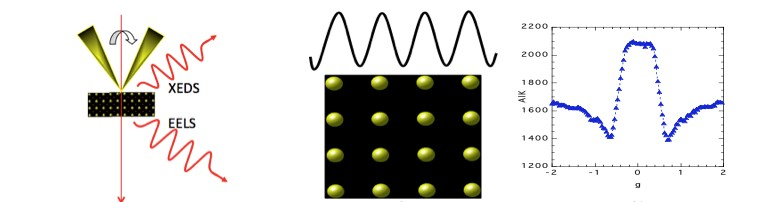
\includegraphics[width=6.5in]{figure1}
	\caption{Times New Roman, 12pt., left-justified. Provide a short description of the figure, including labels and scale markers as appropriate.}
	\label{fig:figure1}
\end{figure}

\begin{figure}[h]
	\centering
	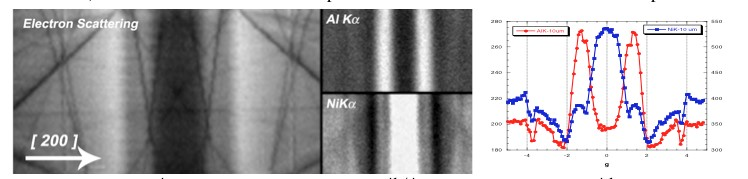
\includegraphics[width=5in]{figure2}
	\caption{Times New Roman, 12pt., left-justified. Provide a short description of the figure, including labels and scale markers as appropriate.}
	\label{fig:figure2}
\end{figure}

\vspace{-1.5em}
\renewcommand{\refname}{\normalsize{References}}
\printbibliography

\end{document}
